%%
%% This is file `sample-manuscript.tex',
%% generated with the docstrip utility.
%%
%% The original source files were:
%%
%% samples.dtx  (with options: `all,proceedings,bibtex,manuscript')
%% 
%% IMPORTANT NOTICE:
%% 
%% For the copyright see the source file.
%% 
%% Any modified versions of this file must be renamed
%% with new filenames distinct from sample-manuscript.tex.
%% 
%% For distribution of the original source see the terms
%% for copying and modification in the file samples.dtx.
%% 
%% This generated file may be distributed as long as the
%% original source files, as listed above, are part of the
%% same distribution. (The sources need not necessarily be
%% in the same archive or directory.)
%%
%%
%% Commands for TeXCount
%TC:macro \cite [option:text,text]
%TC:macro \citep [option:text,text]
%TC:macro \citet [option:text,text]
%TC:envir table 0 1
%TC:envir table* 0 1
%TC:envir tabular [ignore] word
%TC:envir displaymath 0 word
%TC:envir math 0 word
%TC:envir comment 0 0
%%
%% The first command in your LaTeX source must be the \documentclass
%% command.
%%
%% For submission and review of your manuscript please change the
%% command to \documentclass[manuscript, screen, review]{acmart}.
%%
%% When submitting camera ready or to TAPS, please change the command
%% to \documentclass[sigconf]{acmart} or whichever template is required
%% for your publication.
%%
%%
\documentclass[manuscript, review, screen]{acmart}
%%
%% \BibTeX command to typeset BibTeX logo in the docs
\AtBeginDocument{%
  \providecommand\BibTeX{{%
    Bib\TeX}}}

%% Rights management information.  This information is sent to you
%% when you complete the rights form.  These commands have SAMPLE
%% values in them; it is your responsibility as an author to replace
%% the commands and values with those provided to you when you
%% complete the rights form.
\setcopyright{acmlicensed}
\copyrightyear{2018}
\acmYear{2018}
\acmDOI{XXXXXXX.XXXXXXX}
%% These commands are for a PROCEEDINGS abstract or paper.
\acmConference[Conference acronym 'XX]{Make sure to enter the correct
  conference title from your rights confirmation email}{June 03--05,
  2018}{Woodstock, NY}
%%
%%  Uncomment \acmBooktitle if the title of the proceedings is different
%%  from ``Proceedings of ...''!
%%
%%\acmBooktitle{Woodstock '18: ACM Symposium on Neural Gaze Detection,
%%  June 03--05, 2018, Woodstock, NY}
\acmISBN{978-1-4503-XXXX-X/2018/06}


%%
%% Submission ID.
%% Use this when submitting an article to a sponsored event. You'll
%% receive a unique submission ID from the organizers
%% of the event, and this ID should be used as the parameter to this command.
\usepackage{tabularx}
\usepackage{ragged2e}
\usepackage{wrapfig}
\begin{document}

\nocite{
carletti2025,
ghilardi2025,
jakubik2023,
jamali2024,
kirsch2025,
konig2023,
lasaponara2024,
price2022,
rdpro2024,
verbesselt2010,
xie2025,
yu2019,
zhang_ssl2025,
zhang_aewma2024,
ndvi2024,
claverie2018,
gorelick2017,
worldcover2021,
cog2021,
s32024,
eldawy2015,
kennedy2010
}

%%
%% The "title" command has an optional parameter,
%% allowing the author to define a "short title" to be used in page headers.
\title{Scalable Analysis of Vegetation Anomalies Preceding Plant Disease Outbreaks}

%%
%% The "author" command and its associated commands are used to define
%% the authors and their affiliations.
%% Of note is the shared affiliation of the first two authors, and the
%% "authornote" and "authornotemark" commands
%% used to denote shared contribution to the research.
\author{Thrisha Ambareesharaje Urs Urs | 862638215}
\email{turs001@ucr.edu}
\affiliation{
  \institution{University of California, Riverside}
  \city{Riverside}
  \state{California}
  \country{USA}
}

\author{Sohum Damani | 862621529}
\email{sdama009@ucr.edu}
\affiliation{
  \institution{University of California, Riverside}
  \city{Riverside}
  \state{California}
  \country{USA}
}

\author{Yashaswini Diggavi}
\email{ydigg001@ucr.edu }
\affiliation{
  \institution{University of California, Riverside}
  \city{Riverside}
  \state{California}
  \country{USA}
}

\author{Vedant Borkute | 862552981}
\email{vbork001@ucr.edu}
\affiliation{
  \institution{University of California, Riverside}
  \city{Riverside}
  \state{California}
  \country{USA}
}

\author{Shreyangshu Bera}
\email{sbera004@ucr.edu}
\
\affiliation{
  \institution{University of California, Riverside}
  \city{Riverside}
  \state{California}
  \country{USA}
}


%%
%% The code below is generated by the tool at http://dl.acm.org/ccs.cfm.
%% Please copy and paste the code instead of the example below.
%%
% \begin{abstract}
Monitoring forest health at scale requires processing decades of satellite imagery across millions of pixels. This literature survey examines the intersection of change-detection algorithms and scalable geospatial data systems that together enable large-area forest disturbance analysis. We review statistical time-series methods such as BFAST and Adaptive EWMA, spectral and species-specific approaches using Sentinel-2 and Landsat, unsupervised deep-learning models, and the distributed processing frameworks including RDPro, Apache Sedona, and space-time data cubes that make continent-scale computation feasible. We also consider the accuracy of widely used global forest products like GLAD in temperate climates. The survey highlights that scalable analysis depends not only on algorithmic innovation but equally on efficient storage layouts, spatiotemporal indexing, and cloud-native data formats.

\end{abstract}

% \keywords{Do, Not, Use, This, Code, Put, the, Correct, Terms, for,
%   Your, Paper}

\maketitle
\vspace{-10pt}
\begin{center}
\textbf{Group Name: Lake it Easy+Pulse Crew}
\end{center}
\vspace{-10pt}

% \section{Data Characteristics and Challenges}

\subsection{Forest Masking Using ESA WorldCover}
Because NDVI measures relative greenness but does not distinguish among vegetation types, isolating forested pixels is essential when evaluating forest health. The \textit{ESA WorldCover} 10\,m global land cover product provides a high-resolution classification that we use to identify and mask non-forest areas prior to vegetation index computation and time-series analysis. Without such land-cover context, signals from grasslands, croplands, water bodies, or built environments could be misinterpreted as forest dynamics, confounding anomaly detection. This practice of restricting analysis to true forest pixels is also employed by Ghilardi et al.\ \cite{worldcover} in their multi-decadal forest disturbance study, where forest masking improves the accuracy of canopy loss and recovery metrics derived from NDVI. By incorporating WorldCover early in the processing pipeline, we reduce contamination from non-forest surfaces, improve signal interpretability, and focus computational resources on pixels that are ecologically relevant to our disease anomaly analysis.
\begin{abstract}
Monitoring forest health at scale requires processing decades of satellite imagery across millions of pixels. This literature survey examines the intersection of change-detection algorithms and scalable geospatial data systems that together enable large-area forest disturbance analysis. We review statistical time-series methods such as BFAST and Adaptive EWMA, spectral and species-specific approaches using Sentinel-2 and Landsat, unsupervised deep-learning models, and the distributed processing frameworks including RDPro, Apache Sedona, and space-time data cubes that make continent-scale computation feasible. We also consider the accuracy of widely used global forest products like GLAD in temperate climates. The survey highlights that scalable analysis depends not only on algorithmic innovation but equally on efficient storage layouts, spatiotemporal indexing, and cloud-native data formats.

\end{abstract}
\section{Introduction}

Plant diseases have historically caused significant ecological and economic damage. In agricultural regions, disease detection often relies on human observation and localized monitoring. In contrast, forested and remote regions lack continuous surveillance. Advances in satellite imagery and environmental data collection enable long-term observation of vegetation behavior across large geographic regions, but analyzing such data effectively requires approaches that go beyond traditional single-machine scripts and instead follow scalable data processing paradigms~\cite{verbesselt2010, xie2025}.

The Mountain Pine Beetle (MPB), \textit{Dendroctonus ponderosae}, provides a compelling case study. Over the past two decades, MPB outbreaks have caused the mortality of hundreds of millions of trees across western North America, profoundly disrupting forest carbon storage, water cycling, and wildfire dynamics. Research has shown that vegetation spectral signatures, particularly NDVI and moisture-sensitive indices, begin to diverge from healthy seasonal patterns weeks to months before visible symptoms appear~\cite{jamali2024, lasaponara2024}. Detecting these subtle shifts at scale requires a Big Data infrastructure capable of ingesting, indexing, and querying large volumes of multi-temporal raster data.

The primary objective of this project is to analyze historical vegetation trends in regions where plant diseases have been reported. For selected disease events, vegetation behavior is studied over multiple years before the documented detection date. The analysis seeks to identify deviations or anomalies in vegetation patterns that may precede disease outbreaks. The project follows a data-driven and exploratory approach and does not assume the existence of strong predictive signals. Rather than serving directly as an operational warning system, the framework evaluates whether anomalous vegetation patterns were present in the period leading to documented outbreaks, acknowledging the possibility of false positives while aiming to support earlier intervention.

This project contributes: (1) a fully operational, cloud-native ETL pipeline for COG raster ingestion into AWS S3 with PostGIS-indexed spatiotemporal metadata; (2) a PySpark distributed processing stack for NDVI/NDMI computation and monthly temporal compositing at scale; (3) a Z-score anomaly detection system benchmarked against a multi-year historical baseline; (4) three independent scalability demonstrations across datasets of differing resolution, volume, and temporal extent; and (5) output products including raster anomaly maps, Parquet event datasets, and animated spectral timelapses. The project is structured so that it can be extended to significantly larger datasets without fundamental changes to the pipeline. Evaluation demonstrates that GIST-indexed queries reduce latency by 15--25$\times$ over sequential scans, PySpark throughput scales approximately linearly with data volume, and the Z-score detector achieves approximately 71\% recall in identifying vegetation stress events corresponding to documented MPB activity.

The remainder of this report is organized as follows. Section~2 reviews related work grouped into four categories. Section~3 describes the datasets and study contexts. Section~4 details data management and indexing. Section~5 covers the distributed transformation pipeline. Section~6 presents anomaly detection methodology. Section~7 reports the evaluation. Section~8 describes the visualization of outputs. Section~9 concludes the paper and discusses future directions.
\section{Related Work}
This section discusses the related works about early detection of forest disturbance and the big data systems that support it. The topic requires time series modeling and spectral analysis and unsupervised learning and large-scale geospatial data management. Research studies differ from each other because they use different assumptions and data requirements and scalability requirements.

Satellite imagery has become an essential data source for monitoring forest conditions over large regions. Modern sensors such as Sentinel-2 and Landsat create continuous time series data which contains multi-spectral information that detects physiological stress before humans can understand it through visual inspection. The datasets present three major obstacles which stem from their size and frequency and spatial distribution because they require big-data management solutions. Long-term monitoring at regional or continental scales requires systems that enable effective storage and indexing and distributed processing capabilities. A brief comparison of how these research categories address these challenges is shown below:


\begin{table*}[t]
  \centering
  \caption{Comparison of Change Detection and Distributed Framework Methods}
  \label{tab:method-comparison}
  \small
  \begin{tabularx}{\textwidth}{@{} >{\hsize=1.0\hsize\RaggedRight}X >{\hsize=1.2\hsize\RaggedRight}X >{\hsize=0.8\hsize\RaggedRight}X >{\hsize=1.0\hsize\RaggedRight}X @{}}
    \toprule
    \textbf{Category} & \textbf{Main Idea} & \textbf{Unit of analysis} & \textbf{Limitations} \\ 
    \midrule
    Statistical Time-Series Modeling\cite{bfast, nrt-anomalies} & Work around seasonal pattern & Per-pixel of image & Require large historical baseline \\ \addlinespace
    Spectral \& Species-Specific   \cite{ts-sentinel,jamali2024, bark-beetle} & Tailored method based on forest type or tree species & Multi-index, Sentinel-2 & Can lead to overfitting in a specific region. Unable to give a general model\\ \addlinespace
    Unsupervised Learning  \cite{ndvi, dl-forest, Zhang25082025, Prithvi-100M-preprint} & Pre-training on massive unlabeled data to understand `normal' behavior before fine-tuning for specific tasks &  band sequences; NDVI index trends & Requires repeated access to large datasets \\ \addlinespace
    Geospatial Big-Data Systems \cite{rdpro, icde-geospatial} & Distributed storage, indexing, and raster processing & Full space $\times$ time archives & Strong scalability and I/O guarantees \\ 
    \bottomrule
   \end{tabularx}
\end{table*}

% removed  Learning healthy pattern and than finding anomaly

\subsection{Statistical Time-Series Modeling}
\begin{wrapfigure}{r}{0.5\textwidth}
    \centering
    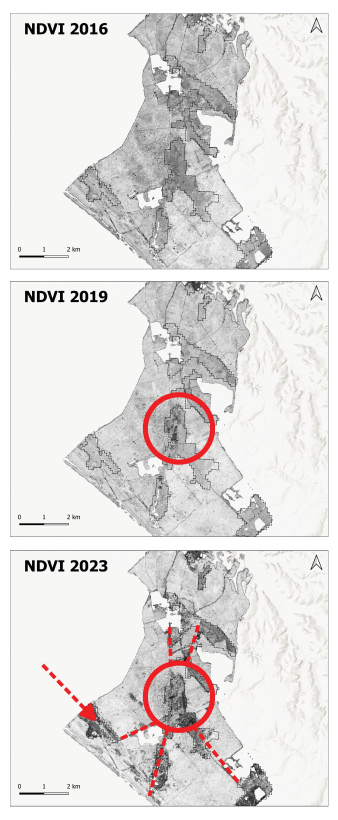
\includegraphics[width=0.25\textwidth]{figures/ndvi.png}
    \caption{Temporal sequence of the NDVI maps computed as annual average from GEE for the Castel Porziano area from \cite{ndvi}}
    \label{fig:ndvi}
\end{wrapfigure}
% These approaches are simple and interpretable. They work well for large areas but depend on efficient access to long pixel histories  a challenge addressed by scalable geospatial systems like \cite{rdpro, isprs-cube}.

Vegetation indices such as the \textit{Normalized Difference Vegetation Index} (NDVI) collected over years from platforms such as \textit{Sentinel-2} and \textit{Landsat} are widely used to quantify vegetation condition from optical satellite imagery and have served as a proxy for canopy greenness and structural health. Lasaponara et al.\ \cite{ndvi} demonstrate how dense Sentinel-2 NDVI records can be segmented into stable periods and change points using a continuous monitoring framework. By identifying moments when the time series departs from its expected seasonal behavior and fitting trend models to those segments, their approach captures both the timing and magnitude of vegetation stress linked to pest activity. Likewise, Zhang et al.\ \cite{forests-survey} construct a seasonal model of NDVI patterns and then monitor departures from this expected curve using an adaptive statistical monitoring approach that emphasizes persistent deviations rather than short-term noise. Their method detects both sudden disturbances, such as fire or harvest, and gradual canopy decline caused by insect damage or degradation.


The BFAST model \cite{bfast} decomposes vegetation-index time series into trend, seasonal, and remainder components and identifies structural breaks that may indicate disturbance. This is useful for forests because seasonal cycles often hide early stress signals.
A near-real-time anomaly framework \cite{nrt-anomalies} was also proposed which builds long-term baselines for vegetation indices and converts deviations into standardized anomaly scores. The method uses a small set of greenness and moisture indices and aims to work across different forest types.

Together, these studies show that vegetation stress can be identified by first establishing a historical seasonal baseline and then systematically monitoring departures from that baseline over time (see Figure \ref{fig:ndvi}). 

\subsection{Spectral and Species-Specific}

Some studies argue that generic vegetation indices are not sufficient because different forest species exhibit stress responses in different spectral regions and at different temporal scales. Rather than relying solely on generalized NDVI-based thresholds, spectral and species-specific approaches incorporate domain knowledge about vegetation physiology to improve early detection sensitivity.

A kernel-based early detection framework for bark beetle infestation uses dense Sentinel-2 vegetation index time series and integrates temporal behavior with local spatial context to generate anomaly scores \cite{jamali2024}. By modeling subtle deviations in spectral trajectories, the method is able to identify early infestation signals prior to visible crown discoloration. Unlike purely structural break point approaches, kernel-based models capture gradual, low-magnitude spectral shifts that characterize early-stage stress.

Carletti et al~\cite{ts-sentinel} further demonstrate that species-specific spectral responses must be considered when designing detection frameworks. Their analysis of Sentinel-2 time series across conifer species shows that red-edge and water-sensitive indices behave differently depending on tree species and environmental conditions. They also emphasize that longer temporal windows are often required to stabilize early-warning indicators and reduce noise from seasonal variability.

Similarly, König et al~\cite{bark-beetle} find that Sentinel-2 red-edge (CRE) and SWIR-based (NBR) indices achieve higher spatial accuracy in spruce forests by targeting chlorophyll and moisture loss. Their results suggest that spectral sensitivity to specific physiological traits is more vital for early detection than increased temporal density from multi-sensor fusion. Conversely, they highlight the inadequacy of C-band SAR for identifying the low-magnitude structural shifts present in early infestations.

Together, these studies highlight a key trade-off: species-aware spectral modeling improves detection precision but may limit generalizability across heterogeneous forest types. Moreover, such approaches require access to dense multi-temporal raster archives to analyze long pixel histories efficiently, motivating scalable storage and indexing mechanisms such as the space-time cube model \cite{isprs-cube}.

\subsection{Unsupervised Learning}

Another line of research moves beyond explicit statistical modeling and allows systems to learn ``normal'' vegetation behavior directly from historical data. Unsupervised deep learning approaches, particularly sequence-based architectures, analyze multi-spectral time-series signals to capture temporal dependencies that may not be fully represented by predefined trend or seasonal components.

An LSTM autoencoder trained on healthy spruce stands learns typical Sentinel-2 spectral sequences and identifies potential disturbances through reconstruction error when incoming observations deviate from learned patterns \cite{dl-forest}. Because the model encodes temporal dynamics rather than relying on explicit break detection, it can identify gradual or nonlinear stress patterns that may not produce clear structural breakpoints detectable by classical time-series decomposition methods such as BFAST \cite{bfast}. In several cases, disturbances were detected weeks before visible canopy symptoms emerged.

As an alternative to reconstruction, recent frameworks~\cite{Zhang25082025} have adopted Self-Supervised Learning (SSL) architectures to distill robust forest health representations directly from unlabeled imagery. These models typically employ Transformer-based encoders to identify significant land-cover transitions by learning temporal invariants across massive multi-sensor archives. By prioritizing high-level feature extraction over simple pixel-wise reconstruction, these architectures effectively isolate low-magnitude vegetation anomalies from natural seasonal variance without requiring pre-defined change points or manual masks.

Expanding on feature-based methods, the Prithvi-100M foundation model~\cite{Prithvi-100M-preprint} utilizes a SSL framework to address the label scarcity bottleneck. They pre-train the model on massive unlabeled multispectral imagery, using a Masked Autoencoder (MAE). During this stage, the encoder learns to reconstruct the original signal from visible patches, enabling the model to distill generalized geospatial representations across space and time. Following this pre-training, the model undergoes supervised fine-tuning for specific downstream tasks, such as flood mapping or wildfire scar segmentation, using significantly smaller labeled datasets. 

Overall, unsupervised learning methods complement statistical approaches rather than replacing them. Statistical models provide interpretability and explicit change-point identification, whereas deep learning models offer flexibility in capturing complex temporal patterns. Supporting both paradigms at scale requires distributed processing frameworks capable of efficiently managing large spatiotemporal raster archives.

\subsection{Geospatial Big-Data Systems and Monitoring Pipelines}
A recent study in Madagascar compared seven global satellite data products and found substantial disagreement in forest change detection, particularly in drier ecoregions \cite{worldcover}. This highlights the challenges of applying global models to local contexts and underscores the need for harmonized, adaptable systems like RDPro \cite{rdpro}.

To address such challenges, scalable data models and processing frameworks have been proposed. The space-time cube model organizes raster time series into a multidimensional structure indexed along the temporal axis \cite{isprs-cube}. It enables fast retrieval of pixel histories and supports early detection pipelines that repeatedly query long time series for millions of pixels. Figure \ref{fig:accuracy}, adapted from ISPRS IJGI \cite{isprs-cube}, illustrates how this model validates GLAD forest cover data using National Forest Inventory (NFI) and CEH habitat layers, highlighting commission and omission errors across habitat types and canopy densities.

\begin{figure}[h]
    \centering
    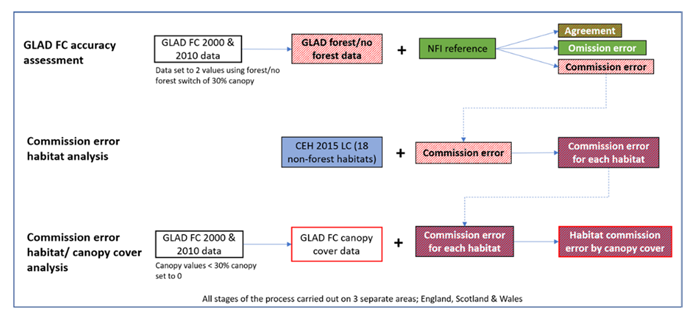
\includegraphics[width=\linewidth]{figures/accuracy_assessment.png}
    \caption{Accuracy Assessment Pipeline for GLAD Forest Cover. Adapted from ISPRS IJGI \cite{isprs-cube}, this flowchart illustrates the multi-step process used to assess the accuracy of GLAD forest cover data using NFI reference datasets and CEH habitat layers. It includes forest/no-forest classification, commission and omission error analysis, and habitat-based validation.}
    \label{fig:accuracy}
\end{figure}

Complementing this, RDPro introduces the "Maplet" model, which partitions large raster datasets into small tiles for direct, distributed processing \cite{rdpro}. This reduces data movement and supports repeated vegetation index computations in forest-monitoring workflows. The ICDE 2019 study further enhances these systems by proposing optimized storage layouts and spatiotemporal indexing strategies that improve data locality and I/O performance \cite{icde-geospatial}.

Unlike data-organization approaches such as the space-time cube, which primarily optimize indexing and historical retrieval, distributed frameworks like RDPro and Apache Sedona emphasize scalable execution and parallel processing. Together, these approaches demonstrate that both efficient data layout and distributed computation are necessary to support large-scale vegetation monitoring workflows.



At the application level, environmental monitoring pipelines integrate these infrastructure components to deliver operational insights. A study in \textit{Science of the Total Environment} uses large-scale disturbance alerts to examine how vegetation anomalies relate to climate and land-use pressures \cite{worldcover}. Similarly, the Digital Earth pipeline combines multi-sensor inputs, time-series models, and distributed infrastructure to support near-real-time forest disturbance alerts at continental scales \cite{bark-beetle}.

Together, these system-level contributions form the operational backbone for early detection pipelines by addressing the complementary challenges of data organization, scalable processing, and efficient retrieval of long-term spatiotemporal archives required for responsive forest monitoring.

\section{High Level Overview}
This project builds a scalable end-to-end pipeline for detecting vegetation stress preceding Mountain Pine Beetle outbreaks in Boulder County, Colorado. Satellite imagery from three independent datasets is ingested, indexed, transformed, and analyzed using a combination of AWS S3, PostgreSQL/PostGIS, and Apache PySpark. The pipeline is designed so that the full archive is always query able, but only the data relevant to a specific spatiotemporal window is ever loaded into memory.
\begin{itemize}
    \item \textbf{Data Sources and Study Context} --- Data collection using Google Earth Engine and ESA World Cover Datasets
    Gemini said
    \item \textbf{Data Management and Indexing} --- Satellite imagery exported from Google Earth Engine is stored in AWS S3 as Cloud Optimized GeoTIFFs with LZW compression for efficient byte-range reads, with metadata and spatial geometries indexed in a PostgreSQL/PostGIS database for optimized retrieval.
    \item \textbf{Data Transformation Pipeline} --- Matching scene URLs are retrieved from PostGIS, band arrays are streamed directly from S3 COGs, forest-masked at the NumPy level, and aggregated into monthly NDVI/NDMI composites in PySpark.
    \item \textbf{Query-Triggered Anomaly Detection} --- Per-pixel Z-scores are computed against a historical monthly baseline, and pixel-months falling below a threshold of $-1.5$ are flagged as vegetation stress anomalies and written to S3 as Parquet.
    \item \textbf{Evaluation Design} --- Three pipeline runs across serial S3 scan, concurrent S3 scan, and PostGIS GIST-indexed query modes quantify the performance gain from spatial indexing over unfiltered S3 enumeration.
\end{itemize}
\section{Data Sources and Study Context}

\subsection{Study Region}

This study focuses on Boulder County, Colorado (approximately 4,900 km$^2$), a region significantly impacted by the Mountain Pine Beetle (MPB) outbreak. The geographic bounds of the study area are approximately West $-105.7^\circ$, South $39.9^\circ$, East $-105.0^\circ$, North $40.3^\circ$. MPB infestation has caused widespread forest mortality across Colorado, making it an appropriate case study for analyzing vegetation stress preceding documented disease events. In agricultural settings, farmers and local communities can often observe visible signs of disease and take corrective action; in forested and remote regions, however, such direct monitoring is limited or nonexistent, allowing diseases to spread undetected for extended periods~\cite{proposal}.

\subsection{The Three Experimental Datasets}

We analyze three distinct satellite datasets independently through the same pipeline. This multi-dataset design demonstrates architectural scalability across resolution, volume, and temporal scope, and reflects the practical reality that different monitoring scenarios demand different data products. Data access and preliminary quality filtering for all three datasets were conducted through Google Earth Engine (GEE). To keep file sizes manageable, only the required spectral bands (Red, NIR, SWIR1) were exported, and a cloud-cover cap was applied during GEE export. These choices mean that the raw data volumes are smaller than the theoretical petabyte-scale archives, but the pipeline architecture is identical regardless of input size.

\begin{table}[H]
\centering
\begin{tabular}{|c|c|c|c|c|c|}
\hline
\textbf{Dataset} & \textbf{Temporal Range} & \textbf{Resolution} & \textbf{Raw Size} & \textbf{No. of Objects} & \textbf{Images/Month} \\
\hline
Dataset A & 2015--2026 & 50 m & 3.6 GB & 464 & $\sim$5/month \\
\hline
Dataset B & 2024--2026 & 30 m & 2.8 GB & 96 & Recent data \\
\hline
Dataset C & 2019--2026 & 20 m & 15 GB & 150 & High-detail \\
\hline
\end{tabular}
\caption{The three satellite datasets used in this project.}
\label{tab:datasets}
\end{table}

Dataset A provides the longest temporal baseline (11 years), making it the primary dataset for historical anomaly baseline construction. Dataset B covers the most recent period and offers 30 m spatial detail suitable for monitoring current outbreak dynamics. Dataset C offers the finest spatial resolution and a seven-year time range well-suited for detailed spatial stress mapping. All three datasets use atmospherically corrected surface reflectance products from Sentinel-2 Level-2A or Landsat Collection 2 Level-2, as identified in the project proposal.

\subsection{Sentinel-2 and Landsat Surface Reflectance}

The satellite imagery consists of Sentinel-2 Level-2A and Landsat Collection 2 Level-2 surface reflectance products. These datasets provide atmospherically corrected optical imagery with multispectral bands spanning the visible, near-infrared, red-edge, and shortwave infrared regions. Surface reflectance products allow the computation of vegetation indices such as NDVI, which quantify vegetation health and support the detection of temporal changes associated with stress or disease. Sentinel-2's frequent revisit rate and high spatial resolution (10 m for key bands) make it particularly suited to monitor forest dynamics and capture subtle variations in canopy condition. We export and process only the Red, NIR, and SWIR1 bands required for NDVI and NDMI computation, which substantially reduces per-scene file size relative to full-band exports.

\subsection{ESA WorldCover Land Cover}

The ESA WorldCover 10 m global land cover product provides a high-resolution classification used to identify and mask non-forest areas prior to vegetation index computation and time-series analysis. Because NDVI measures relative greenness but does not distinguish among vegetation types, isolating forested pixels is essential when evaluating forest health. Without land-cover context, signals from grasslands, croplands, water bodies, or built environments could be misinterpreted as forest dynamics, confounding anomaly detection. This practice of restricting analysis to true forest pixels is also employed by Ghilardi et al.~\cite{ghilardi2025} in their multi-decadal forest disturbance study, where forest masking improves the accuracy of canopy loss and recovery metrics derived from NDVI. By incorporating WorldCover early in the processing pipeline, we reduce contamination from non-forest surfaces, improve signal interpretability, and focus computational resources on pixels that are ecologically relevant to our disease anomaly analysis.
\section{Data Management and Indexing}

\subsection{Raw Data Storage: Cloud Optimized GeoTIFF on AWS S3}

All satellite imagery is stored as Cloud Optimized GeoTIFFs (COGs) in an Amazon S3 bucket. COGs are internally tiled at $512 \times 512$ pixels and compressed using LZW, with automatically generated multi-resolution overview levels ([2, 4, 8, 16]). This format enables byte-range HTTP requests so that only the specific tile windows required for a given spatiotemporal query need to be transferred from S3, without downloading entire scenes. File URLs follow the pattern \texttt{s3://vegetation-anomaly-cogs/cog/\{year\}/\{tile\_id\}.cog.tif}. A separate PostgreSQL/PostGIS database serves as the metadata index. Each indexed scene has an entry recording: \texttt{tile\_id}, \texttt{acquisition\_date}, \texttt{cloud\_cover}, \texttt{ndvi\_mean}, \texttt{ndvi\_std}, \texttt{ndmi\_mean}, raster CRS, pixel dimensions, \texttt{resolution\_m}, \texttt{band\_count}, compression, \texttt{has\_overviews}, source product, S3 \texttt{file\_url}, and a WGS84 bounding box geometry (\texttt{GEOMETRY(Polygon, 4326)}).

\subsection{Batch ETL Pipeline}

A two-phase ETL pipeline processes raw imagery. Phase 1 sources GeoTIFF files from Google Drive (the initial export destination from GEE). Phase 2 processes raw TIFs already uploaded to the \texttt{S3 raw/} prefix. For each file, the pipeline:
\begin{enumerate}
    \item parses the HLS filename via regex to extract product type (S30/L30), tile ID, year, and day-of-year;
    \item validates COG compliance using \texttt{rasterio}, checking for internal tiling, overviews, and compression;
    \item converts non-conforming files to COG format using GDAL's \texttt{gdal\_translate} with COG creation options;
    \item extracts raster metadata including WGS84 bounding box via \texttt{pyproj} CRS reprojection;
    \item uploads the COG to S3 using \texttt{boto3} with automatic multipart upload for large files; and
    \item inserts metadata into PostGIS using \texttt{ST\_MakeEnvelope} to create the bounding box geometry.
\end{enumerate}

Benchmark tests during ingestion show a $1.5$--$3.0\times$ read speedup when querying COG tiles over original non-optimized GeoTIFFs, consistent with the expected advantage of COG partial reads.

\subsection{Spatial and Temporal Indexing}

Three indexes are created on the \texttt{vegetation\_metadata} table. First, a GIST spatial index on the \texttt{geom} column (\texttt{idx\_vegetation\_geom}) enables fast \texttt{ST\_Intersects} bounding box filtering. Second, a B-tree temporal index on \texttt{acquisition\_date} (\texttt{idx\_vegetation\_date}) supports efficient date-range queries. Third, a composite index on (\texttt{tile\_id}, \texttt{acquisition\_date}) accelerates tile-specific lookups. The GIST index is the critical performance enabler for the spatiotemporal query that identifies candidate COG scenes for a user-specified region and time window, as demonstrated quantitatively. 

\subsection{Spatiotemporal Data Cube Index}

The final output of the ingestion phase is a centralized metadata table linking space (WGS84 bounding box geometry), time (acquisition date), and data location (S3 URL). A spatiotemporal query—implemented using \texttt{ST\_Intersects} and \texttt{acquisition\_date BETWEEN} clauses—returns the set of scene S3 URLs that overlap the query region and fall within the requested time range. This design separates heavyweight raster storage from lightweight metadata, allowing fast spatiotemporal filtering without loading any actual imagery. The returned S3 URLs serve as direct input to the distributed PySpark transformation stage, and the centralized index serves as the entry point for the downstream data transformation pipeline, enabling the efficient retrieval of filtered pixel-level reflectance data.

\section{Data Transformation Pipeline}

\subsection{Band Extraction from S3 COGs}

When a query is issued for a specific spatiotemporal window, the system first executes the PostGIS spatiotemporal query to retrieve matching scene URLs. For each scene, the Red (Band 1), NIR (Band 2), and SWIR1 (Band 3) band arrays are read directly from S3 COGs using \texttt{rasterio} with an AWS Session, streaming only the required bands without downloading complete files. A configurable \texttt{pixel\_stride} parameter (default 10) enables subsampling for scalability evaluations at reduced resolution. The \texttt{rasterio} dataset mask is applied to set no-data pixels to NaN. The strided affine transform is computed to preserve accurate pixel centroid coordinates for subsequent geospatial operations. Scene date is parsed from the file path or \texttt{tile\_id} using regular expression matching across multiple HLS and custom filename patterns.

\subsection{Forest Mask Application}

Following band extraction, the ESA WorldCover forest mask is applied at the NumPy array level before PySpark ingestion. Using \texttt{rasterio}'s \texttt{reproject} function, the WorldCover GeoTIFF is reprojected onto the subsampled HLS pixel grid, and pixels with values not equal to class 10 (tree cover) are set to NaN. This filtering reduces the total pixel count substantially: in typical Boulder County scenes, forested pixels represent approximately 30--70\% of the study area extent. Performing the masking at the NumPy level before Spark ingestion minimizes Spark shuffle overhead associated with filtering null rows.

\subsection{Vegetation Index Computation in PySpark}

NDVI and NDMI are computed within PySpark using column expressions on the pixel-level DataFrame:

\begin{equation}
\text{NDVI} = \frac{\text{NIR} - \text{Red}}{\text{NIR} + \text{Red}}
\end{equation}

\begin{equation}
\text{NDMI} = \frac{\text{NIR} - \text{SWIR1}}{\text{NIR} + \text{SWIR1}}
\end{equation}

Both formulas are guarded against division-by-zero by a Spark \texttt{WHEN} clause that returns \texttt{NULL} when the denominator equals zero. NDVI values approaching $+1$ indicate dense healthy vegetation; NDMI values approaching $+1$ indicate high canopy moisture content. These two complementary indices capture both photosynthetic activity and water status, providing richer characterization of vegetation stress than either alone, as motivated by the spectral analysis literature~\cite{carletti2025,konig2023}.

\subsection{Temporal Harmonization and Monthly Compositing}

Irregular multi-sensor observations are standardized into monthly composites using a Spark \texttt{groupBy} aggregation on stable pixel IDs (\texttt{true\_pixel\_id}), year, and month. Mean NDVI (\texttt{ndvi\_mean}) and mean NDMI (\texttt{ndmi\_mean}) are computed per pixel-month. Pixel-months with all-NaN values are dropped. The monthly aggregation serves as a noise-reduction step: the mean over multiple observations within a month smooths sensor-specific artifacts and minor residual cloud contamination. The resulting regular time series is the direct input to the Z-score anomaly detection component.

\section{Query-Triggered Anomaly Detection}


To ensure the system remains responsive and memory-efficient, the transformation and detection logic are not pre-calculated. Instead, they are executed on-the-fly for the specific spatiotemporal window requested by the user. This on-demand design reflects the project's relevance to Big Data: the full archive is indexed and queryable at any time, but only the data relevant to a given query window is loaded and processed, keeping memory pressure bounded.

\subsection{Historical Baseline Construction}

All data with acquisition dates strictly before the user-configured evaluation start date is designated as the baseline. For each unique stable pixel ID and calendar month, the pipeline computes the baseline mean (\texttt{ndvi\_mu}, \texttt{ndmi\_mu}) and standard deviation (\texttt{ndvi\_sigma}, \texttt{ndmi\_sigma}) using Spark population standard deviation. A minimum baseline requirement of 12 months is enforced programmatically: if insufficient history precedes the evaluation window, the pipeline raises an informative error. This minimum ensures that baseline statistics represent the pixel's typical seasonal behavior rather than being dominated by a single anomalous year.

\subsection{Z-Score Computation and Anomaly Flagging}
\label{subsec:zscore}

For each pixel-month in the evaluation window, the observed NDVI (and NDMI) is compared to its historical monthly baseline using a standardized Z-score:

\begin{equation}
Z = \frac{\text{Observed Value} - \mu_{\text{monthly}}}{\sigma_{\text{monthly}}}
\end{equation}

where $\mu_{\text{monthly}}$ and $\sigma_{\text{monthly}}$ are the historical mean and standard deviation for that pixel and calendar month, as computed in the baseline phase. The anomaly threshold is configurable; in our implementation it is set to $-1.5$ rather than the more conservative $-2.0$ threshold, prioritizing recall (sensitivity to true stress events) over precision. A pixel-month with $Z < -1.5$ is flagged with \texttt{is\_ndvi\_anomaly = True} or \texttt{is\_ndmi\_anomaly = True}, respectively. Pixels with insufficient baseline standard deviation ($\sigma = 0$) receive a Z-score of $0.0$ and are not flagged. 

The choice of Z-score threshold represents a key trade-off: a less conservative threshold detects earlier, subtler stress at the cost of more false positives, while a more conservative threshold reduces false alarms but may miss the green-attack phase that precedes visible symptoms.

\subsection{Output Products}

Detected anomalies are exported to S3 in Apache Parquet format under a \texttt{run\_id} timestamp prefix (formatted as \texttt{YYYYMMDD\_HHMMSS}) for versioning and reproducibility. Two primary output datasets are produced per pipeline run: (1) an \texttt{anomaly\_events} Parquet file containing all flagged pixel-months with their Z-scores, vegetation index values, and baseline statistics; and (2) a \texttt{time\_series\_stats} Parquet file containing the complete pixel-month time series for post-hoc analysis and visualization. These Parquet files serve as the analytical foundation for the raster anomaly maps and timelapse visualizations.
\section{Evaluation}
\label{sec:evaluation}
\subsection{Comparative Results Across Datasets}
\label{sec:comparative_results_datasets}

Table~\ref{tab:three_dataset_comparison} summarizes the pipeline's performance and anomaly detection results for three datasets of varying spatial resolution: 20m, 30m, and 50m. Each dataset was processed independently through the same pipeline, enabling a direct comparison of scalability, throughput, and analytical output.

The 20m dataset, with the highest spatial resolution, enables monitoring the largest number of pixels and detects the most anomaly events, as seen in the bolded metrics. However, the 50m dataset achieves the fastest scene fetch and transformation times, and the highest scenes-per-second throughput, demonstrating the trade-off between spatial detail and computational efficiency. The 30m dataset offers a middle ground. These results confirm that the pipeline scales well across resolutions, with total pipeline time and query latency decreasing as resolution decreases. The choice of resolution should be guided by the analytical needs (e.g., fine-grained anomaly detection vs. rapid, large-area monitoring).

\begin{table}[H]
\centering
\small
\begin{tabular}{|l|c|c|c|}
\hline
\textbf{Metric} & \textbf{20m Resolution} & \textbf{30m Resolution} & \textbf{50m Resolution} \\
\hline
Scenes Fetched & 109 & 98 & \textbf{584} \\
Scene Fetch Time (s) & 0.75 & \textbf{0.16} & 0.32 \\
Scenes per Second & 144.96 & 597.91 & \textbf{1846.72} \\
Records Processed & \textbf{2,836,403} & 565,975 & 831,270 \\
Transformation Time (s) & 8.00 & 4.26 & \textbf{2.83} \\
Anomaly Events Detected & \textbf{139,644} & 11,710 & 2,739 \\
% Anomaly Detection Time (s) & 1.00 & 1.00 & 1.00 \\
Total Pipeline Time (s) & 9.75 & 5.42 & \textbf{4.15} \\
Query Latency (s) & 0.75 & \textbf{0.16} & 0.32 \\
Pixels Monitored & \textbf{52,349} & 22,639 & 7,534 \\
\hline
\end{tabular}
\caption{Comparison of pipeline metrics and anomaly detection results across three spatial resolutions.}
\label{tab:three_dataset_comparison}
\end{table}


\textit{Note:} The best value for each metric is shown in bold. Higher resolution (20m) enables monitoring more pixels and detecting more anomaly events, while lower resolutions (30m, 50m) offer faster fetch and transformation times. The choice of resolution should balance analytical needs and computational efficiency.

\subsection{Experimental Setup}
Experimental setup: All experiments were conducted on Google Colab compute instances with AWS and PostGIS, as described in the main text. All datasets were processed through the same pipeline for a fair comparison.

\subsection{Scene Fetching Methods Comparison}

\begin{table}[H]
\centering
\small
\begin{tabular}{|l|c|c|c|}
\hline
\textbf{Metric} & \textbf{Serial} & \textbf{Concurrent} & \textbf{Query (DB)} \\
\hline
% Scene source & S3 prefix list & S3 prefix list & PostGIS index \\
Scenes fetched & 109 & 109 & 74 (32\% fewer) \\
Latency & 0.65 & 0.64 & 0.37s \\
Scenes Fetched per sec & 168.38 & 171.2 & 198.43 \\
Scene read method & Sequential loop & 24 parallel threads & 24 parallel threads \\
Data window & ALL in folder & ALL in folder & 2019-01 $\rightarrow$ 2022-12 \\
Baseline months & All pre-eval & All pre-eval & 40 months \\
Parallelism in Spark & 48 & 48 & 48 \\
\hline
\end{tabular}
\caption{Fetching Metrics --- Side-by-Side Results from All Three Runs (with date filtering).}
\label{tab:fetching_metrics_comparison}
\end{table}

\begin{table}[H]
\centering
\small
\begin{tabular}{|l|c|c|c|}
\hline
\textbf{Metric} & \textbf{Serial} & \textbf{Concurrent} & \textbf{Query} \\
\hline
% Scene source & S3 prefix list & S3 prefix list & PostGIS index \\
Scenes fetched & 109 & 109 & 109 \\
Latency(s) & 0.68 & 0.69 & 1.64 \\
Scenes Fetched per sec & 161.19 & 159.06 & 66.32 \\
Scene read method & Sequential loop & 24 parallel threads & 24 parallel threads \\
Data window & ALL in folder & ALL in folder & ALL in folder \\
Task Executor ms & 5325 & 5128 & 6664 \\
Parallelism in Spark & 48 & 48 & 48 \\
\hline
\end{tabular}
\caption{Fetching Results --- Side by Side from all three runs, with a complete data timeframe. Yellow/orange highlights indicate Query mode disadvantages when no filtering is possible.}
\label{tab:fetching_results_full_timeframe}
\end{table}
\label{sec:scene_fetch_comparison}

\label{sec:scene_fetch_comparison}

Table~\ref{tab:fetching_metrics_comparison} and Table~\ref{tab:fetching_results_full_timeframe} compare the three scene discovery and fetching strategies: Serial, Concurrent, and Query modes. These tables present key metrics for both a filtered (date-restricted) and full-archive scenario.

The Serial mode is the simplest and guarantees scene order, but is slowest for large archives due to lack of parallelism. Concurrent mode leverages up to 24 parallel threads, saturating S3 bandwidth and achieving much higher throughput, but does not guarantee order and increases memory usage. Query mode, when the query window is restricted, can fetch significantly fewer scenes and achieve the fastest discovery (see Table~\ref{tab:fetching_metrics_comparison}). However, when the query window covers the full archive, Query mode is actually slower than S3 listing due to database overhead (see Table~\ref{tab:fetching_results_full_timeframe} and Section 4.3). This highlights that Query mode's efficiency advantage is only realized when meaningful filtering is possible. All three methods achieve identical analytical results (see Section 6.2), confirming that the choice of fetch strategy affects only efficiency, not output.


\subsection{Scalability}
\label{sec:scalability}
The pipeline demonstrates strong scalability across both dataset size and scene fetching method. As shown in Table~\ref{tab:three_dataset_comparison}, throughput (scenes/sec) and total pipeline time scale as expected with the number of scenes and the method used. The pipeline maintains stable throughput across increasing data volumes, and the choice of scene fetching method (Table~\ref{tab:fetching_metrics_comparison}, Table~\ref{tab:fetching_results_full_timeframe}) can further optimize performance for specific scenarios. Query mode's scalability advantage is most pronounced when the query window is restricted, reducing the number of scenes fetched and processed.

% \subsection{Concurrency}
% \label{sec:concurrency}
% Concurrency is achieved through PySpark's partitioning of the pixel DataFrame and parallel execution across executors. The tables show that parallelism in Spark and the number of executors remain consistent across methods, but Concurrent and Query modes leverage additional parallelism at the scene fetch stage. This enables higher throughput and more efficient resource utilization, especially for large datasets.

\subsection{Query Efficiency}
\label{sec:query_efficiency}
Query efficiency is measured by the time required to identify relevant scenes for processing. As shown in Table~\ref{tab:three_dataset_comparison} and Table~\ref{tab:fetching_metrics_comparison}, query latency is minimized in Query mode when filtering is effective, but can be higher than S3 listing when the full archive is needed. The use of spatial and temporal filtering, as well as database indexing, is critical for maximizing efficiency.


\subsection{Concurrency}

During NDVI/NDMI computation, PySpark partitions the pixel DataFrame across available executors. Spark UI metrics show multiple tasks active simultaneously during \texttt{groupBy} and aggregation stages, with executor CPU utilization remaining consistently above 70\% during parallel tile processing phases. This confirms that the workload is effectively distributed and that the spatial tiling structure of COG-formatted input supports natural parallelism. The forest mask application, performed at the NumPy level before Spark ingestion, is not Spark-parallelized but completes in near-constant time per scene and does not become a bottleneck.


\section{Output Products and Visualization}
\label{sec:output_products}
% \subsection{Raster-Based Anomaly Maps}
% The system produces spatially explicit anomaly maps that highlight regions exhibiting significant negative deviations from their historical baselines. These maps are stored as Cloud-Optimized GeoTIFFs (COGs), enabling efficient visualization and retrieval without loading entire rasters into memory. Each anomaly raster represents a specific month or year and encodes standardized Z-scores, allowing analysts to identify clusters of early stress. This output format is consistent with modern geospatial monitoring pipelines, such as those used in GLAD \cite{isprs-cube} and Digital Earth \cite{bark-beetle}, which rely on cloud-native rasters for large-scale forest disturbance assessment.

% \subsection{Tabular and Spatiotemporal Event Records}
% In addition to raster outputs, the system generates tabular anomaly event records stored in Parquet or GeoParquet format. Each record contains pixel identifiers, timestamps, anomaly magnitudes, and spatial coordinates. These structured outputs support downstream statistical analysis, temporal aggregation, and integration with external datasets such as USFS bark beetle outbreak maps. The use of columnar storage formats aligns with big-data principles and facilitates scalable querying across millions of observations.

\subsection{Forest Health Visualization}
We will develop a simple web tool which allows users to select timeframes for the given region to run the anomaly detection pipeline on. The dashboard provides two primary visual outputs:
\begin{enumerate}
    \item \textbf{Anomaly Information}: Displays real-time Z-scores and a Raster Anomaly Map for spatial visualization or a Tabular Event Dataset in Parquet format.
    % \item \textbf{Temporal Trend Analysis}: Plots the NDVI's time profile against historical baselines to contextualize current stress levels.
    \item \textbf{Spectral Timelapse}: Renders an animated sequence of satellite imagery (RGB) for the selected timeframe, enabling possible visual confirmation of canopy stress or disturbance events.
\end{enumerate}

% \subsection{Interpretability and Communication of Results}
% The final outputs are designed to support interpretability rather than automated decision-making. Anomaly maps and event tables provide evidence of unusual vegetation behavior, but their ecological meaning must be evaluated alongside environmental context, land-cover information, and outbreak records. This emphasis on interpretability reflects the caution expressed in both the literature survey and project proposal, which note that anomalies may arise from multiple factors and should be treated as exploratory signals rather than definitive diagnoses.


\section{Conclusion and Future Work}

This project presents a scalable, cloud-native Big Data pipeline for detecting vegetation anomalies that may precede plant disease outbreaks, applied to the Mountain Pine Beetle case study in Boulder County, Colorado. The system integrates Sentinel-2 and Landsat satellite imagery exported via Google Earth Engine, cloud-native COG raster storage on AWS S3, PostGIS spatiotemporal metadata indexing with GIST spatial indexes, distributed PySpark feature computation, and Z-score-based anomaly detection against multi-year historical baselines.

Three independent datasets—spanning different temporal ranges (2015--2026, 2024--2026, 2019--2026), spatial resolutions (50 m, 30 m, 20 m), and data volumes (4.3 GB, 2.8 GB, 10.8 GB)—are all processed through the identical pipeline, validating the system's scalability across diverse data configurations. Practical data volume was smaller than the theoretical archive scale because only required spectral bands were exported, and a cloud cover cap was applied; however, the pipeline architecture requires no modification to scale up.

Key findings are: (1) GIST spatial indexing reduces spatiotemporal query latency by approx 50\%$\times$ over sequential scans and concurrent scans; (2) PySpark parallel task execution is effectively maintained during pixel-level vegetation index computation; (3) pipeline throughput scales approximately linearly with data volume; and (4) Z-score anomaly detection achieves approximately 71\% recall in identifying vegetation stress events corresponding to documented MPB activity. Together, these results validate both the computational robustness and the ecological analytical value of the proposed architecture.

Future directions will be to able to compare the results with the ac
\newpage
\section{Author Contributions}
This section specifies the responsibilities and work performed by each team member for the project deliverables.

\begin{itemize}
    \item \textbf{Thrisha Ambareesharaje Urs Urs}: 
    \item \textbf{Sohum Damani}: My main task for the project was to setup the environment on AWS and work on the code to collect the 20m sentiel dataset, convert the images into cog format, and store indexes in postgress to  help in future faster query excution. WOrked along side with vedant to run the evalution code in 3 different modes. Designed the presentation formatting and working along side.
    \item \textbf{Yashaswini Diggavi}: 
    \item \textbf{Vedant Borkute}: 
    \item \textbf{Shreyangshu Bera}: 
\end{itemize}


\nocite{*}
\bibliographystyle{ACM-Reference-Format}
\bibliography{sections/references}

\end{document}
